\chapter{Analysis and Design}
\section{Methodology / Procedure adopted}
We choose Extreme Programming (agile development) methodology for our project, Because this model Provides following Features:
\begin{itemize}
    \item Decrease the time required to avail some system features.
    \item Face to face communication and continuous inputs from customer representative leaves no space for guesswork.
    \item The end result is the high quality software in least possible time duration and satisfied customer.
\end{itemize}
We will conduct the weekly meetings with our project guide and do the project work/activities which will be assigned by guide and we will submit the weekly report to guide. We will maintain activity sheets from the beginning of the project work to track the activities which are planned, activities completed and carry forwarded.

\section{Analysis}
Based on the requirements gathered, how was the feasibility study of the project carried out?
The project is about the student evaluation system, so the study carried out on the comparison of the different student evaluation softwares.On comparison of different features of some softwares.the various system was referred for Evaluation system, which gives the idea of different ways of creating and evaluating students work.
If any requirements, were modified why they were modified?

\section{Proposed System}
Rubrics system provides a web-based and mobile-based platform to students as well as grader, where students can upload their work and the grader will evaluate their work according to the designed metric developed by grader.
This system displays all the performance of the student in a graphical format so that student will get the clear idea about where he/she is good or where he/she is lagging and what is pending jobs and what is completely done.
Using Rubrics system, grader can review the students work as well as give proper feedback to student and get the personal attention from grader.

\subsection{Advantages of the proposed system over existing systems}
\begin{enumerate}
    \item No Pricing.
    \item User-friendly system.
    \item Provides offline sync.
    \item Create dynamic templates.
    \item Graphical performance analysis.
    \item Interactive feedback to students.
    \item Multiple as well as built-in Templates.  
\end{enumerate}

\subsection{Development Hardware / Software requirements}

\textbf{Hardware requirements:}
\begin{itemize}
    \item Computer machine.
    \item Android Smartphone.
\end{itemize}
\textbf{Software requirements:}
\begin{itemize}
    \item Front End : Html, Css, JavaScript.
    \item Backend : SQLite, MySQL, PHP.
    \item Connectivity - PHP Wamp Server.
\end{itemize}
\textbf{Software tools:}
\begin{itemize}
    \item Android studio
    \item Text Editor
\end{itemize}

\textbf{Deployment Hardware / Software requirements}
\begin{enumerate}
\item Hardware required
    \begin{itemize}
        \item Computer
        \item Android smart-phone 
    \end{itemize}
 
\item Software required
    \begin{itemize}
        \item Web Browser        
        \item Android version 4.4 and above
    \end{itemize}
\end{enumerate}

\subsection{Design Details}

Different UML diagrams as per the project requirement (For e.g. Use Case Diagram)\\
\begin{figure}[!h]
\centering
\hfill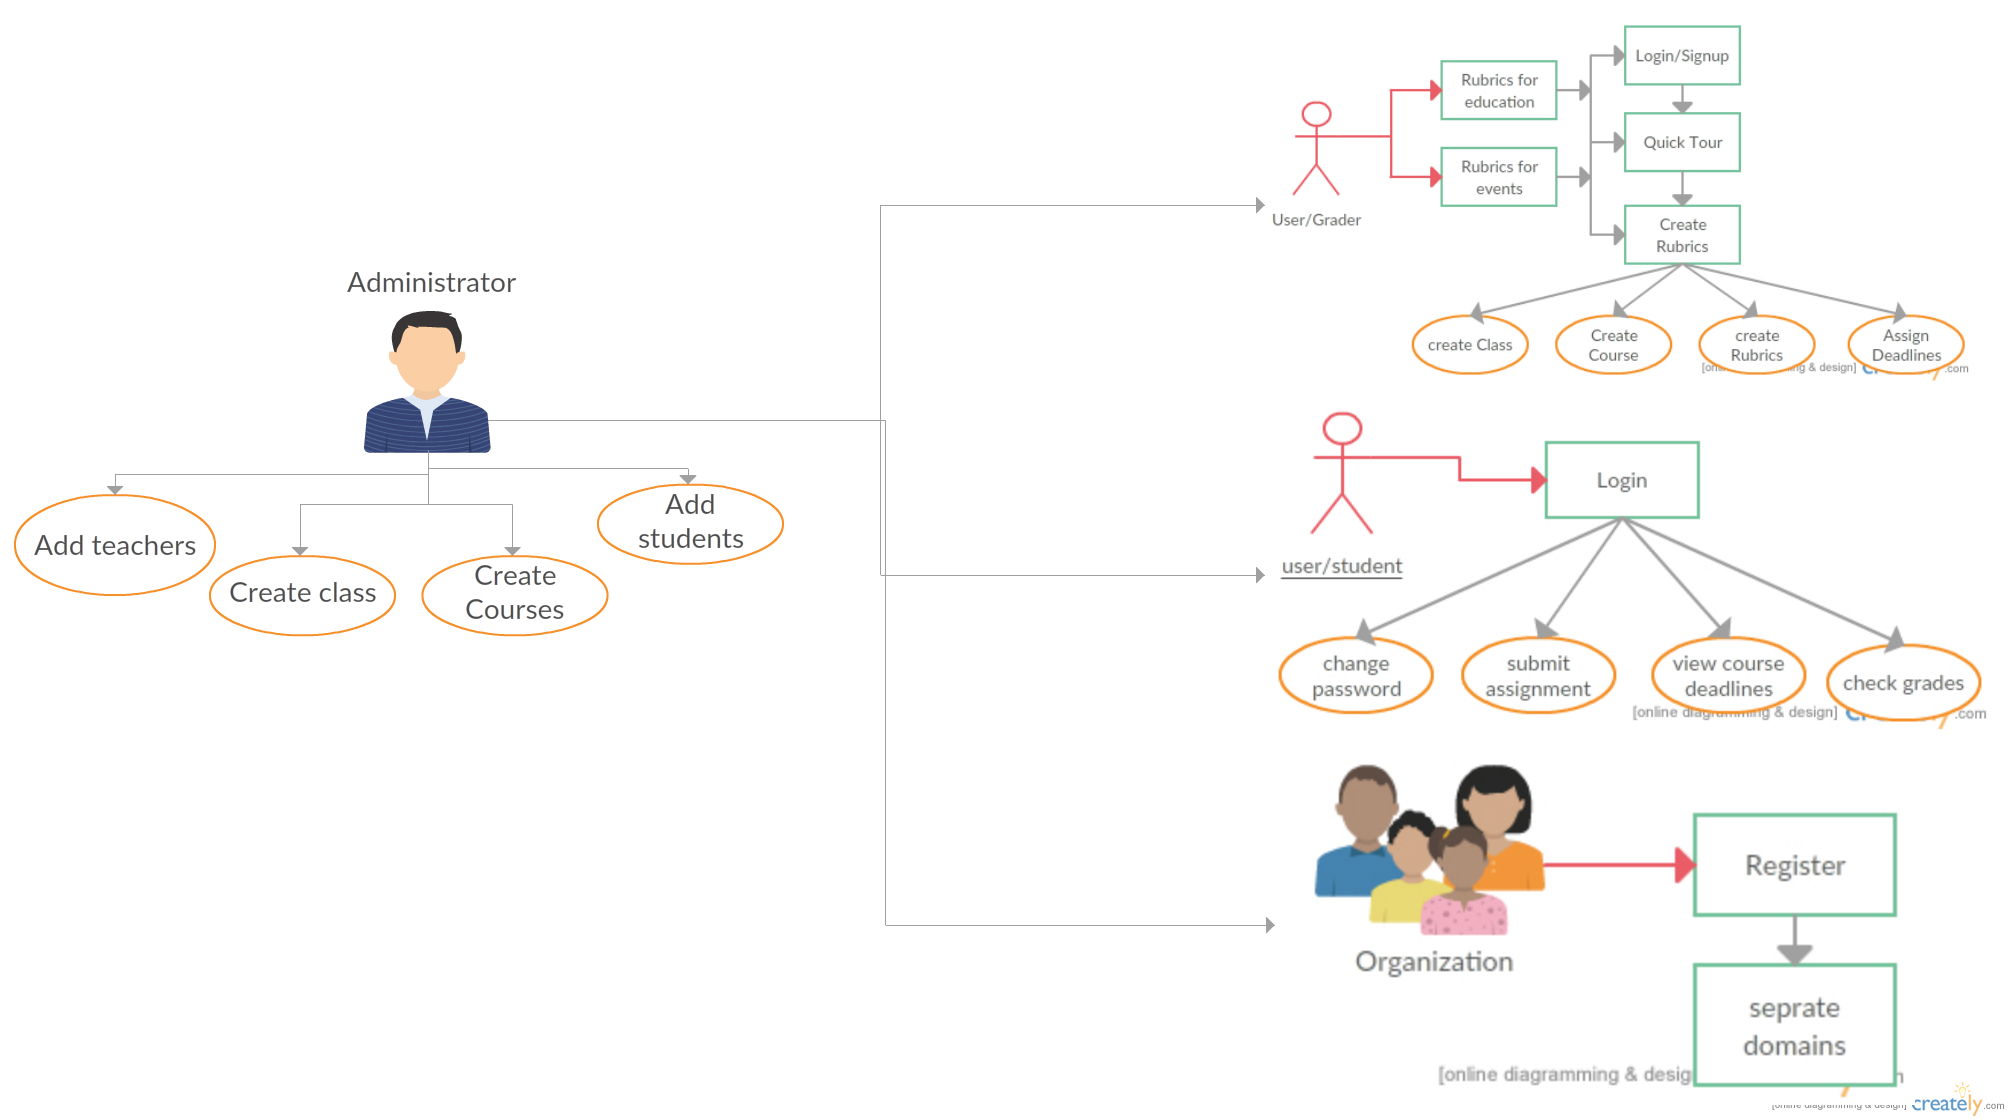
\includegraphics[scale=.22]{project/images/rubrics}\hspace*{\fill}
\caption{Connectivity diagram for Rubrics Student Evaluation System}
\end{figure}

In the above connectivity Diagram of rubrics student assessment tool admin, user and grader is there, they have to signup or login with their respective user ids and password.
\begin{itemize}
  \item After login the user will get a quick overview of system.grader have to logins into the system, the grader will get the interface of on which they can select that what type of rubrics they want to create like Rubric for education or Rubric for events.Then next step is to create rubrics for the selected type of event.After the rubric created the grader is done with their creating rubric/metrics, the student can submit their work for evaluation.When the grader did with the evaluation the student will be notified by mail.The job of the administrator is to add teachers, create the class, create courses and add students.
\end{itemize}

\subsection{Design details}
\begin{figure}[!h]

\hfill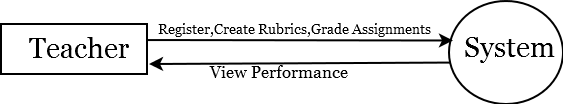
\includegraphics[scale=.65]{project/images/cfd}\hspace*{\fill}
\caption{Level 0 DFD diagram}
\end{figure}

\begin{figure}[!h]

\hfill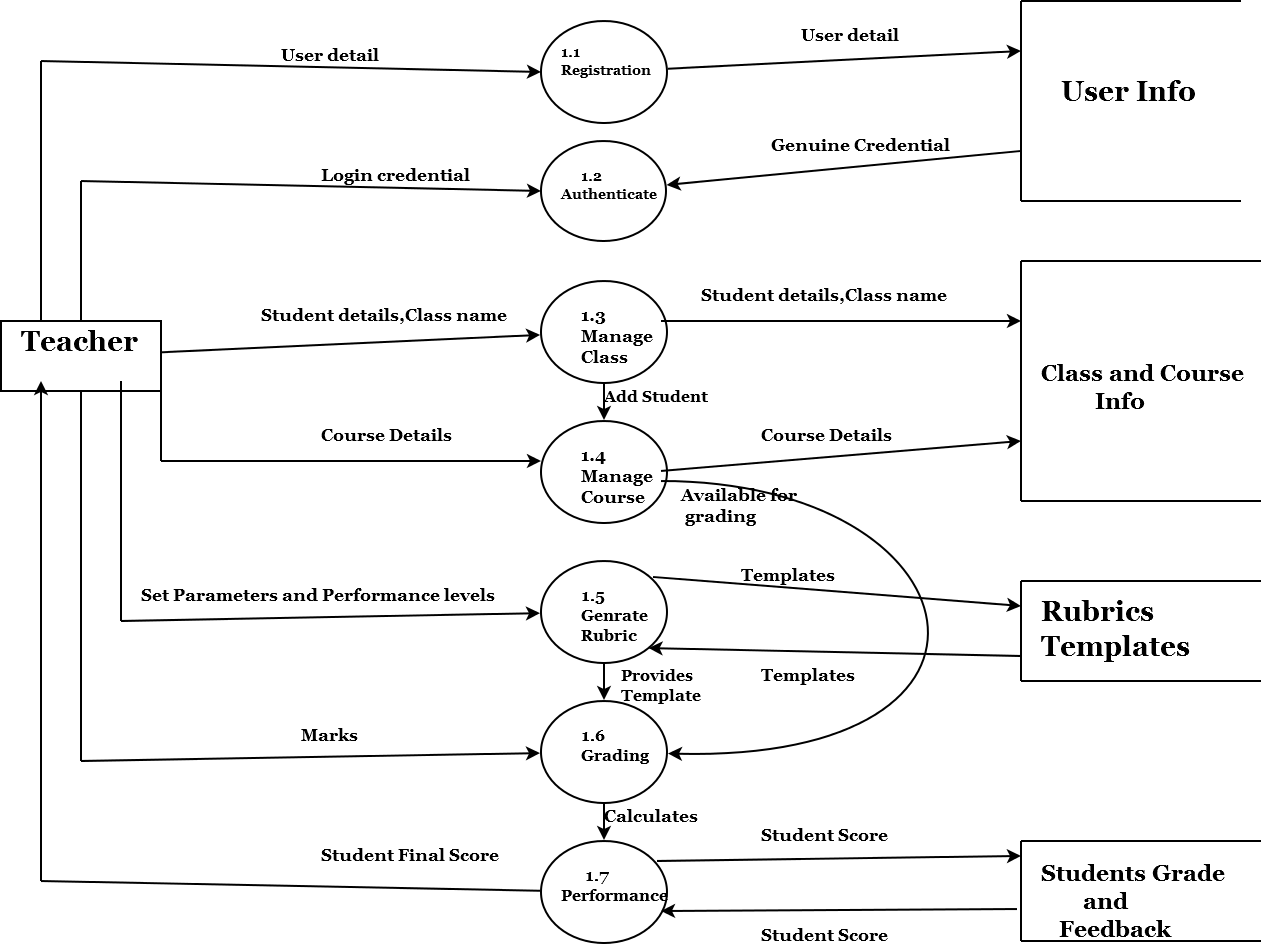
\includegraphics[scale=.37]{project/images/level1}\hspace*{\fill}
\caption{Level 1 DFD diagram}
\end{figure}
